%%%%%%%%%%%%%%%%%%%%%%%%%%%%%%%%%%%%%%%%%
% Short Sectioned Assignment
% LaTeX Template
% Version 1.0 (5/5/12)
%
% This template has been downloaded from:
% http://www.LaTeXTemplates.com
%
% Original author:
% Frits Wenneker (http://www.howtotex.com)
%
% License:
% CC BY-NC-SA 3.0 (http://creativecommons.org/licenses/by-nc-sa/3.0/)
%
%%%%%%%%%%%%%%%%%%%%%%%%%%%%%%%%%%%%%%%%%

%----------------------------------------------------------------------------------------
%	PACKAGES AND OTHER DOCUMENT CONFIGURATIONS
%----------------------------------------------------------------------------------------

\documentclass[paper=a4, fontsize=11pt]{scrartcl} % A4 paper and 11pt font size

\usepackage{listings}
\usepackage{color}

\definecolor{dkgreen}{rgb}{0,0.6,0}
\definecolor{gray}{rgb}{0.5,0.5,0.5}
\definecolor{mauve}{rgb}{0.58,0,0.82}

\lstset{frame=tb,
language=Java,
aboveskip=3mm,
belowskip=3mm,
showstringspaces=false,
columns=flexible,
basicstyle={\small\ttfamily},
numbers=none,
numberstyle=\tiny\color{gray},
keywordstyle=\color{blue},
commentstyle=\color{dkgreen},
stringstyle=\color{mauve},
breaklines=true,
breakatwhitespace=true,
tabsize=3
}

\usepackage[T1]{fontenc} % Use 8-bit encoding that has 256 glyphs
\usepackage[utf8]{inputenc}
\usepackage[spanish]{babel} % English language/hyphenation
\usepackage{amsmath,amsfonts,amsthm} % Math packages
% \usepackage{breakcites}
\usepackage{sectsty} % Allows customizing section commands
\allsectionsfont{\centering \normalfont\scshape} % Make all sections centered, the default font and small caps
\usepackage{algorithm}
\usepackage{url}
\usepackage[noend]{algpseudocode}
\makeatletter
\usepackage{graphicx}

\usepackage{fancyhdr} % Custom headers and footers
\pagestyle{fancyplain} % Makes all pages in the document conform to the custom headers and footers
\fancyhead{} % No page header - if you want one, create it in the same way as the footers below
\fancyfoot[L]{} % Empty left footer
\fancyfoot[C]{} % Empty center footer
\fancyfoot[R]{\thepage} % Page numbering for right footer
\renewcommand{\headrulewidth}{0pt} % Remove header underlines
\renewcommand{\footrulewidth}{0pt} % Remove footer underlines
\setlength{\headheight}{13.6pt} % Customize the height of the header
% Reinsert missing \algbackskip
\def\algbackskip{\hskip-\ALG@thistlm}
\renewcommand*{\ALG@name}{Algoritmo}
% \makeatother
\decimalpoint
\numberwithin{equation}{section} % Number equations within sections (i.e. 1.1, 1.2, 2.1, 2.2 instead of 1, 2, 3, 4)
\numberwithin{figure}{section} % Number figures within sections (i.e. 1.1, 1.2, 2.1, 2.2 instead of 1, 2, 3, 4)
\numberwithin{table}{section} % Number tables within sections (i.e. 1.1, 1.2, 2.1, 2.2 instead of 1, 2, 3, 4)

\setlength\parindent{0pt} % Removes all indentation from paragraphs - comment this line for an assignment with lots of text

%----------------------------------------------------------------------------------------
%	TITLE SECTION
%----------------------------------------------------------------------------------------

\newcommand{\horrule}[1]{\rule{\linewidth}{#1}} % Create horizontal rule command with 1 argument of height

\title{	
\normalfont \normalsize 
\textsc{Universidad Nacional de San Agustín, Escuela de Ingenieria de Sistemas} \\ [25pt] % Your university, school and/or department name(s)
\horrule{0.5pt} \\[0.4cm] % Thin top horizontal rule
\huge ADA - Lab 03 \\ % The assignment title
\horrule{2pt} \\[0.5cm] % Thick bottom horizontal rule
}

\author{Fernando Enrique Araoz Morales - 20173373} % Your name

\date{\normalsize\today} % Today's date or a custom date

\begin{document}

\maketitle % Print the title

%----------------------------------------------------------------------------------------
%	PROBLEM 1
%----------------------------------------------------------------------------------------

\section{Introducción}\label{sec:introducción}

En el presente documento se presenta un análisis del tiempo de ejecución del algoritmo Closest Pair,
así como las respuestas a otras interrogantes relacionadas.

\section{Implementación}\label{sec:implementación}

La implementacion del algoritmo inicia por la definición de una clase Coordenada. Esta tiene como
únicos atributos un entero denotando una posicion x, y otro para una posicion y.
Estos son finales y protegidos para así evitar toda la ceremonia de crear getters, setters, y
manejar el state.


\begin{lstlisting}

    class Coordinate {
        final int x;
        final int y;

        Coordinate(int x, int y) {
            this.x = x;
            this.y = y;
        }

    }

\end{lstlisting}

Luego, la implementación de la clase propiamente dicha. Esta consta de los métodos run y describe
requeridos por la interfaz IAlgorithm, así como métodos para el cálculo del algoritmo con fuerza
bruta y eficientemente, un método para clonar ArrayList, y otro para separar y ordenar el ArrayList.

\begin{lstlisting}

    public class ClosestPairProblem implements IAlgorithm {

        private ArrayList<Coordinate> coordinates;
        double result;

        ClosestPairProblem(ArrayList<Coordinate> coordinates) {
            this.coordinates = coordinates;
        }

        @Override
        public boolean run() {
            result = calc();
            return true;
        }

        double calc() {
            int size = coordinates.size();
            ArrayList<Coordinate> coordinates_x = extractElements(coordinates, 0, size);
            coordinates_x.sort((c1, c2) -> c1.x - c2.x);
            ArrayList<Coordinate> coordinates_y = extractElements(coordinates, 0, size);
            coordinates_y.sort((c1, c2) -> c1.y - c2.y);
            return efficientClosestPair(coordinates_x, coordinates_y);
        }

        private double bruteForceClosestPair(ArrayList<Coordinate> coordinates) {
            double minimunDistance = Double.MAX_VALUE;

            for (int i = 0; i < coordinates.size(); i++) {
                Coordinate c1 = coordinates.get(i);
                for (int j = i + 1; j < coordinates.size(); j++) {
                    Coordinate c2 = coordinates.get(j);
                    double distance = Math.sqrt(
                        Math.pow(c1.x - c2.x, 2) +
                        Math.pow(c1.y - c2.y, 2)
                    );
                    minimunDistance = Math.min(minimunDistance, distance);
                }
            }

            return minimunDistance;
        }

        private ArrayList<Coordinate> extractElements(ArrayList<Coordinate> elements,
                int start, int end) {
            ArrayList<Coordinate> result = new ArrayList<>();
            for (int i = start; i < end; i++) {
                result.add(elements.get(i));
            }
            return result;
        }

        private double efficientClosestPair(ArrayList<Coordinate> coordinates_x,
                ArrayList<Coordinate> coordinates_y) {
            if (coordinates_x.size() <= 3) return bruteForceClosestPair(coordinates_x);

            int size = coordinates_x.size();
            int half_limit = (int) Math.ceil(coordinates_x.size() / 2);
            ArrayList<Coordinate> c_x_left = extractElements(coordinates_x, 0, half_limit);
            ArrayList<Coordinate> c_y_left = extractElements(coordinates_y, 0, half_limit);

            ArrayList<Coordinate> c_x_right = extractElements(coordinates_x, half_limit, size);
            ArrayList<Coordinate> c_y_right = extractElements(coordinates_y, half_limit, size);

            double minimum_left  = efficientClosestPair(c_x_left, c_y_left);
            double minimum_right = efficientClosestPair(c_x_right, c_y_right);

            double minimum = Math.min(minimum_left, minimum_right);
            Coordinate mediumPoint = coordinates_y.get(half_limit - 1);

            ArrayList<Coordinate> mediumElements = new ArrayList<>();
            for (Coordinate c: coordinates_x) {
                if (Math.abs(c.x - mediumPoint.x) < minimum) {
                    mediumElements.add(c);
                }
            }

            double dminsq = minimum * minimum;

            for (int i = 0; i < mediumElements.size() - 2; i++) {
                int k = i + 1;
                Coordinate c1 = mediumElements.get(i);
                Coordinate c2 = mediumElements.get(k);
                double value = Math.pow(c1.y - c2.y, 2);
                while (k <= size - 1 && value < dminsq) {
                    double result = Math.pow(c1.x - c2.x, 2) + Math.pow(c1.y - c2.y, 2);
                    dminsq = Math.min(result, dminsq);
                    k++;
                }
            }

            return Math.sqrt(dminsq);
        }

        @Override
        public String description() {
            return "Calculates the closes pair from a list of coordinates.";
        }

    }

\end{lstlisting}

    Esta implementación sigue como base aquella brindada en clase. Algunas peculiaridades son que
    para satisfacer la interfaz IAlgorithm, el método run() simplemente ejecuta el método calc(),
    y almacena el resultado de este en la propiedad de clase resultado, la cual el usuario deberá
    usar.

    El método calc() clona el ArrayList brindado via constructor en uno ordenado según el eje x y
    otro ordenado según el eje y. Para realizar el ordenamiento se utilizó el método sort de
    ArrayList, y expresiones lambda.

\section{Tiempo de ejecución}\label{sec:tiempos-de-ejecución}

El algoritmo, debido a su implementación, tiene un tiempo de ejecución corto. Con 100 elementos
tarda 71ms, con 1000 elementos tarda 76ms, con 10000 tarda 116ms, con 100000 elementos
aumenta a 360ms, y con 1000000 elementos alcanza los 1531ms.

\section{Gráficos}\label{sec:gráficos}

Los gráficos del plano se encuentran a continuación:

\begin{figure}
    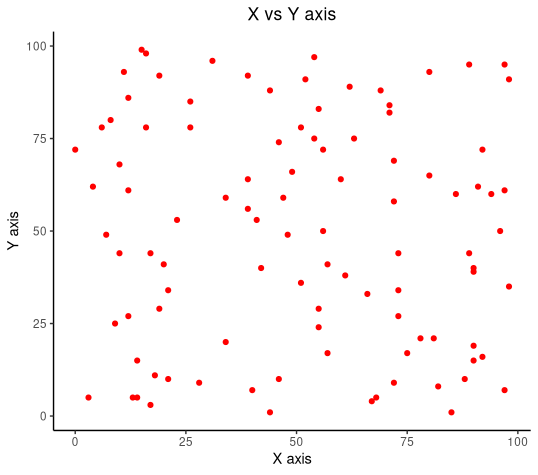
\includegraphics[width=\linewidth]{Rplot1.png}
    \caption{100 elementos.}
\end{figure}



\begin{figure}
    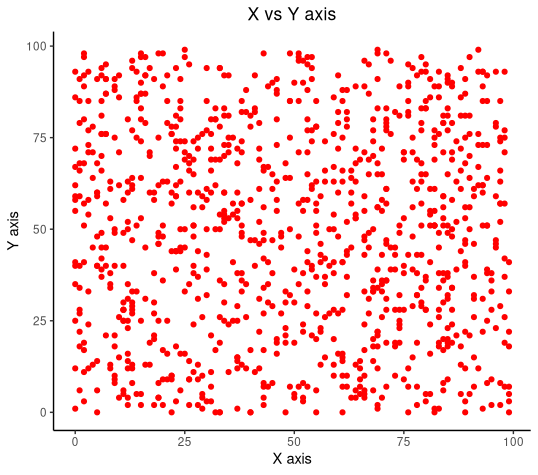
\includegraphics[width=\linewidth]{Rplot2.png}
    \caption{1000 elementos.}
\end{figure}



\begin{figure}
    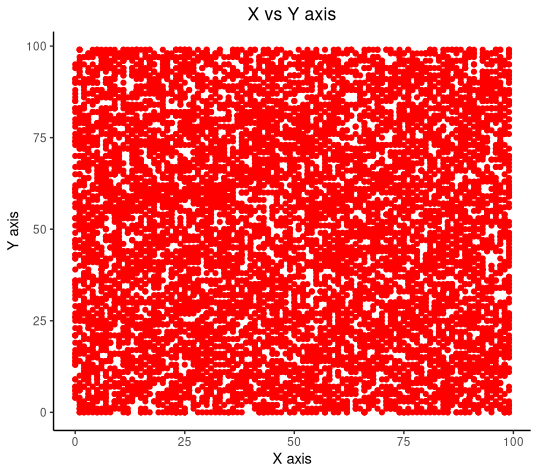
\includegraphics[width=\linewidth]{Rplot3.png}
    \caption{10000 elementos.}
\end{figure}



\begin{figure}
    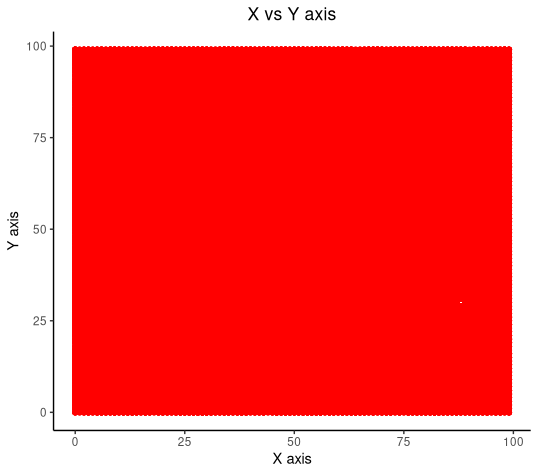
\includegraphics[width=\linewidth]{Rplot4.png}
    \caption{100000 elementos.}
\end{figure}

\section{Descripción de los gráficos}\label{sec:descripción-de-los-gráficos}

A partir de los gráficos provistos anteriormente, y usando como referencia el tiempo de ejecución
del algoritmo, podemos observar que a pesar de que la cantidad de elementos en cada caso
aumenta de manera muy significativa, el tiempo de ejecución no lo hace, indicando una vez más
la eficiencia del algorítmo.

\section{Límite de puntos para comparación entre fuerza bruta y divide y venceras.}\label{sec:comparación-entre-fuerza-bruta-y-divide-y-venceras.}

En el pseudocódigo brindado en clase este límite se establece en 3 elementos. Sin embargo, es
posible aumentar este sin afectar fuertemente el rendimiento a una gran escala. Hay que notar,
sin embargo, que la diferencia de rendimiento es cuadrático vs n log n, por lo que se busca es
minimizar este límite al máximo.

\section{Costo usando teorema maestro}\label{sec:costo-usando-teorema-maestro}

El costo se puede calcular de la siguiente manera:

T(n) = 2T(n/2) + O(n) + O(nLogn) + O(n)

T(n) = 2T(n/2) + O(nLogn)

T(n) = T(n x Logn x Logn)


En este caso tomamos como base un algoritmo de ordenamiento de orden O(n log n).


%------------------------------------------------

\end{document}